\documentclass[border=10pt]{standalone}
\usepackage[svgnames]{xcolor}
\usepackage{amsmath}
\usepackage{pgfplots}
\pgfplotsset{compat=newest}
\usepackage[sfdefault]{FiraSans}
\usepackage{FiraMono}
\renewcommand*\familydefault{\sfdefault}
\begin{document}
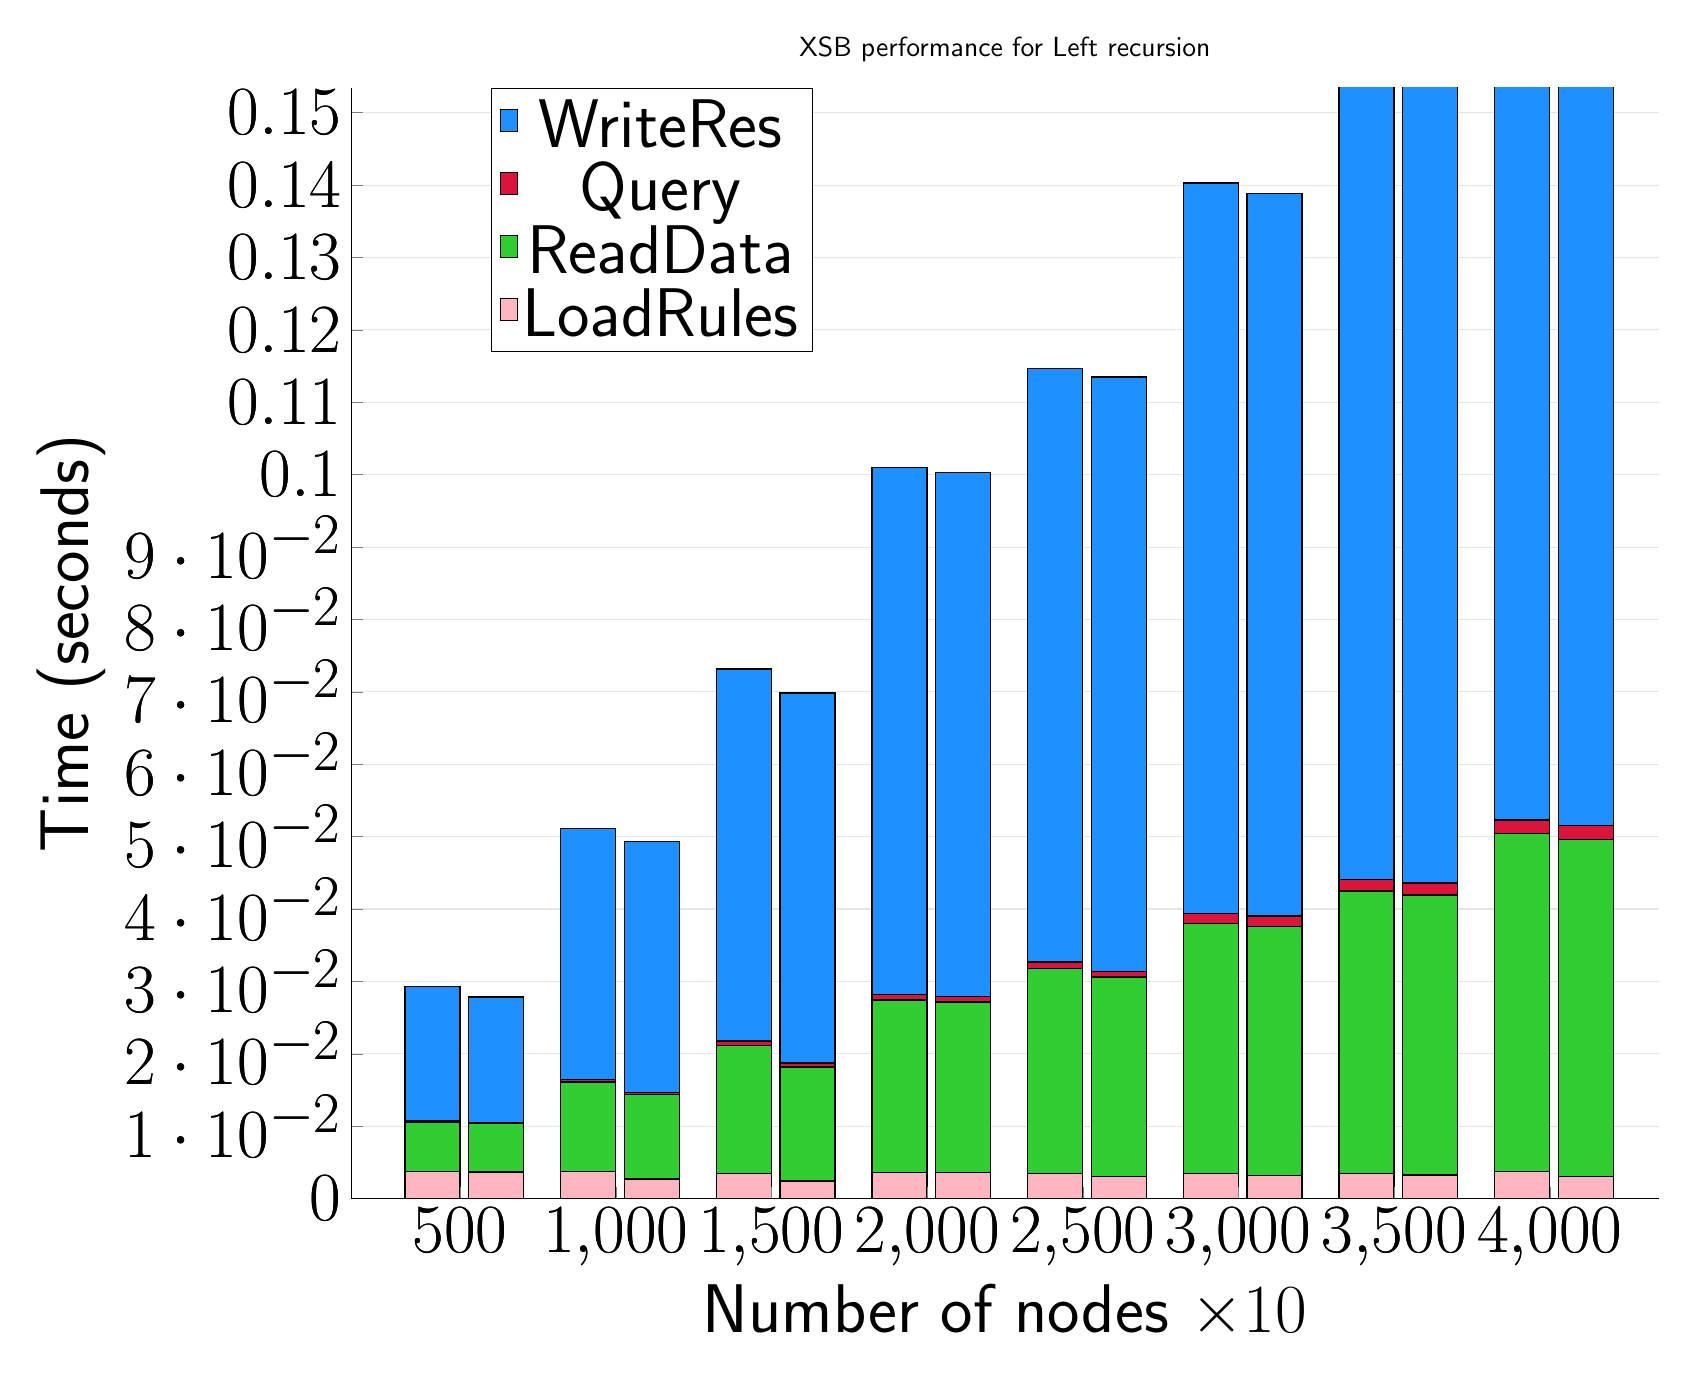
\begin{tikzpicture}
\begin{axis}[
   ybar stacked,
   title={XSB performance for Left recursion},
   bar shift=-10pt,
   width=1.5\textwidth,
   bar width=0.7cm,
   ymajorgrids, tick align=inside,
   major grid style={draw=gray!20},
   xtick=data,
   ymin=0, ymax=0.15343540827433244,
   axis x line*=bottom,
   axis y line*=left,
   enlarge x limits=0.1,
   legend style={
       at={(0.23, 1)},
       anchor=north,
       legend columns=1,
       font=\Huge,
   },
   ylabel={Time (seconds)},
   xlabel={Number of nodes $\times 10$},
   label style={font=\Huge},
   tick label style={font=\Huge},
]
\addlegendimage{fill=DodgerBlue, draw=black, line width=0.2pt}
\addlegendentry{WriteRes}
\addlegendimage{fill=Crimson, draw=black, line width=0.2pt}
\addlegendentry{Query}
\addlegendimage{fill=LimeGreen, draw=black, line width=0.2pt}
\addlegendentry{ReadData}
\addlegendimage{fill=LightPink, draw=black, line width=0.2pt}
\addlegendentry{LoadRules}
\addplot +[fill=LightPink, draw=black, line width=0.5pt] coordinates {
    (500, 0.00370335578918457)
    (1000, 0.0036969979604085297)
    (1500, 0.003478050231933597)
    (2000, 0.00362666447957357)
    (2500, 0.00348798433939616)
    (3000, 0.0034387906392415366)
    (3500, 0.00348369280497233)
    (4000, 0.0037103494008382198)
};
\addplot +[fill=LimeGreen, draw=black, line width=0.5pt] coordinates {
    (500, 0.006887276967366536)
    (1000, 0.012421925862630199)
    (1500, 0.017693281173706034)
    (2000, 0.023811340332031264)
    (2500, 0.028267939885457366)
    (3000, 0.03451697031656903)
    (3500, 0.038987318674723305)
    (4000, 0.04670842488606774)
};
\addplot +[fill=Crimson, draw=black, line width=0.5pt] coordinates {
    (500, 0.000191370646158854)
    (1000, 0.000340700149536133)
    (1500, 0.000581979751586914)
    (2000, 0.0007930596669514976)
    (2500, 0.0009393692016601554)
    (3000, 0.0014613469441731768)
    (3500, 0.0016289552052815733)
    (4000, 0.0019019444783528634)
};
\addplot +[fill=DodgerBlue, draw=black, line width=0.5pt] coordinates {
    (500, 0.018507003784179712)
    (1000, 0.034623384475708)
    (1500, 0.051408052444458015)
    (2000, 0.07277727127075197)
    (2500, 0.08194295565287275)
    (3000, 0.10087601343790716)
    (3500, 0.13157812754313106)
    (4000, 0.13343540827433245)
};
\end{axis}
\begin{axis}[
   ybar stacked,
   bar shift=13pt,
   width=1.5\textwidth,
   bar width=0.7cm,
   ymajorgrids, tick align=inside,
   major grid style={draw=none},
   xtick=data,
   ymin=0, ymax=0.15343540827433244,
   axis x line*=none,
   axis y line*=none,
   enlarge x limits=0.1,
   label style={font=\Huge},
   tick label style={font=\Huge},
]
\addplot +[fill=LightPink, draw=black, line width=0.5pt] coordinates {
    (500, 0.0036773333333333332)
    (1000, 0.002721333333333333)
    (1500, 0.002425333333333334)
    (2000, 0.0036076666666666666)
    (2500, 0.003024)
    (3000, 0.0032133333333333337)
    (3500, 0.003251)
    (4000, 0.0030779999999999996)
};
\addplot +[fill=LimeGreen, draw=black, line width=0.5pt] coordinates {
    (500, 0.006654333333333334)
    (1000, 0.011632666666666666)
    (1500, 0.015775)
    (2000, 0.02353066666666667)
    (2500, 0.027585666666666665)
    (3000, 0.03433733333333333)
    (3500, 0.038688)
    (4000, 0.046556999999999994)
};
\addplot +[fill=Crimson, draw=black, line width=0.5pt] coordinates {
    (500, 0.00018966666666666936)
    (1000, 0.00029099999999999965)
    (1500, 0.0005363333333333354)
    (2000, 0.0007926666666666663)
    (2500, 0.0007770000000000011)
    (3000, 0.0014613333333333334)
    (3500, 0.0016293333333333368)
    (4000, 0.0019020000000000068)
};
\addplot +[fill=DodgerBlue, draw=black, line width=0.5pt] coordinates {
    (500, 0.017303333333333327)
    (1000, 0.034654333333333336)
    (1500, 0.05112866666666666)
    (2000, 0.07234666666666667)
    (2500, 0.08211666666666666)
    (3000, 0.099814)
    (3500, 0.13112333333333334)
    (4000, 0.13222466666666668)
};
\end{axis}
\end{tikzpicture}

\end{document}
